\section{Code}
GitHub IPDMP Repository Link: \url{https://github.com/nicoarrroyo/IPDMP}

\subsection{NALIRA Code Walk-through}
\subsubsection{Preliminaries}
This initial phase involves importing necessary libraries (os, numpy, csv, PIL, time, custom modules like \verb|data_handling|, \verb|image_handling|, misc, \verb|user_interfacing|), defining global constants and settings (DPI for plots, number of chunks, resolution choice, plotting/saving flags, data filename), and setting up the home directory path based on the operating environment (personal PC vs. university machine). It also records the start time for performance tracking.

\subsubsection{Initial Image Handling}
This section focuses on locating and loading the required Sentinel-2 spectral band image files.

\textbf{File Paths}: It constructs the full paths to the necessary band image files (.jp2 format) based on the satellite name, number, specific image folder name, and the chosen resolution ('10m' or '60m'). It handles Sentinel-2's specific folder structure, including navigating the 'GRANULE' subdirectories and selecting the appropriate resolution folders ('R10m', 'R20m', 'R60m'). It uses helper functions (\verb|get_sentinel_bands|) to determine the correct band identifiers (e.g., 'B03' for Green, 'B08' for NIR at 10m). For high-resolution processing, it combines paths from both R10m and R20m folders as needed (e.g., SWIR bands are only available at 20m).

\textbf{Converting Image to Array}: The \verb|image_to_array| function (from \verb|image_handling.py|) is used to open each specified band image file and convert its pixel data into a NumPy array. For high-resolution mode where bands have different native resolutions (10m and 20m), lower-resolution arrays (20m SWIR1, SWIR2) are upscaled later during cloud masking using \verb|upscale_image_array| to match the 10m resolution arrays before index calculation. The resulting arrays are stored in a list.

\subsubsection{Cloud Masking}
This step aims to remove cloud-contaminated pixels from the band image arrays. It uses the Sentinel 2 Cloud Probability mask file (\verb|MSK_CLDPRB_20m.jp2| or \verb|MSK_CLDPRB_60m.jp2|). 
\begin{itemize}
    \item The appropriate resolution cloud mask file is opened and converted to a NumPy array using \verb|image_to_array|.
    \item If high-resolution bands are used, the 20m cloud mask is upscaled by a factor of 2 (\verb|upscale_image_array|) to match the 10m band resolution. The 20m SWIR1 and SWIR2 band arrays are also upscaled here.
    \item Pixels in the cloud mask array with a probability value greater than 50 are set to 100.
    \item The coordinates (indices) of these high-probability cloud pixels are identified using \verb|np.argwhere|.
    \item These coordinates are then used to set the corresponding pixel values in all the loaded band image arrays (Blue, Green, NIR, SWIR1, SWIR2) to 0, effectively masking them out before index calculation.
\end{itemize}
The images have to be upscaled for NALIRA because the final two items in the \verb|image_arrays| list are the \verb|swir1| and \verb|swir2| arrays, which have the lower \verb|20m| spatial resolution. However, for KRISP, this becomes a problem because the \verb|image_arrays| only contains \verb|green| and \verb|NIR|, which have \verb|10m| spatial resolution. Upscaling these images creates an oversized \verb|ndwi| array which would produce mini-chunks that are double the size of what KRISP was trained on. To prevent this, there is a check in \verb|mask_sentinel| which verifies that the length of the \verb|image_arrays| list is greater than or equal to three, in which case the band images are upscaled as normal, and if this is not the case, then only the cloud array is upscaled. 

\subsubsection{Calculating Water Indices}
With the cloud-masked (and potentially upscaled) band arrays ready, this section calculates various water indices.
\begin{itemize}
    \item The NumPy arrays, initially of type \verb|uint16|, are converted to integer type (\verb|astype(int)|) to prevent overflow issues during calculations.
    \item The required bands are unpacked: Blue, Green, NIR, SWIR1, SWIR2.
    \item NumPy's error settings are adjusted to ignore division by zero and invalid value errors that can occur during index calculation (e.g., division by zero if both bands are zero).
    \item All four indices discussed in the methodology (NDWI, MNDWI, AWEI-SH, and AWEI-NSH) are calculated pixel-wise using standard formulas. 
    \item The resulting index arrays (NDWI, MNDWI, AWEI-SH, AWEI-NSH) are stored in a list.
\end{itemize}

\subsubsection{Note on Varying Resolutions}
The images generated by combining 10m and 20m resolution data can appear to have a slightly higher effective resolution than pure 20m images due to the way these indices are calculated. For indices requiring bands of different native resolutions—such as MNDWI, AWEI-SH, and AWEI-NSH—the lower resolution 20m bands (like SWIR1, SWIR2, and the 20m cloud mask) are upscaled to match the 10m resolution of bands such as Blue, Green, and NIR. During this process, each pixel from the 20m image effectively becomes four pixels, as both the height and width are doubled, ensuring that pixel-wise operations are compatible before performing the index calculations (see step 3.3.3).

% !!!!! PLACEHOLDER !!!!!
\begin{figure}[ht]
    \centering
    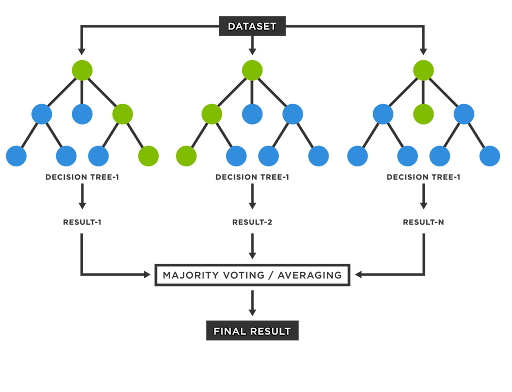
\includegraphics[width=0.6\textwidth]{contents/figures/LR RF diagram.jpg}
    \caption{SVM Confusion Matrix \citep{maity_2016}}
    \label{fig:NOTHING}
\end{figure}
% !!!!! PLACEHOLDER !!!!!

This means that for the calculation of MNDWI, for example, although four pixels of SWIR1 will all have the same value (because they have effectively been 'quadruplicated' to fit the same size array) the four pixels of Green will have the same resolution they had before, meaning they may change slightly from pixel to pixel. This has the effect of creating 2x2 pixel boxes of similar colours because only one of the two bands are changing in value, while the other stays stagnant, effectively limiting the maximum range of change within these boxes. 

\subsubsection{Displaying Indices}
This optional step visualizes the calculated water index arrays using Matplotlib.
\begin{itemize}
    \item It checks the \verb|show_index_plots| flag. If \verb|False|, the step is skipped.
    \item If \verb|True|, it iterates through the calculated index arrays (NDWI, MNDWI, AWEI-SH, AWEI-NSH).
    \item For each index, it creates a \verb|matplotlib| figure (\verb|plt.figure|) and displays the index array as an image (\verb|plt.imshow|).
    \item A title indicating the satellite, index name, DPI, and resolution is added. Axis labels and ticks are hidden for clarity.
    \item It checks the \verb|save_images| flag. If \verb|True|, the plot is saved as a PNG file (\verb|plt.savefig|) with a descriptive name, handling potential duplicate filenames by appending a counter.
    \item The plot is displayed on the screen ('plt.show').
\end{itemize}

\subsubsection{Data File Preparation}
This section prepares the CSV file used to store the manual labels.
\begin{itemize}
    \item It defines the path for the labelling data, creating the 'training data' subdirectory if it doesn't exist using \verb|change_to_folder|.
    \item The target CSV filename (\verb|responses_<n_chunks>_chunks.csv|) is defined.
    \item \verb|blank_entry_check| is called to remove any empty rows from the CSV file, ensuring data integrity. \verb|check_file_permission| is called within \verb|blank_entry_check| to avoid errors if the file is open elsewhere.
    \item File Validity Check: The script reads the existing CSV file (if any) and checks for validity. It verifies that the first column (chunk number) increments sequentially. If inconsistencies (e.g., missing chunks, incorrect order) or formatting errors are found, it prompts the user to retry, create a new file ('new'), or quit ('quit'). If a new file is created, it writes the header row and a dummy first entry.
    \item Data Completion Check: After validating the sequence, it checks if existing entries are complete. It iterates through the rows, verifying that if a row indicates the presence of reservoirs (column 1 \textgreater 0) or water bodies (column 2 \textgreater 0), the corresponding coordinate columns (column 3 onwards for reservoirs, column 8 onwards for bodies) actually contain coordinate data (identified by starting with '['). It also flags rows where coordinates exist but the count is zero. If incomplete or inconsistent rows are found, it sets a \verb|data_correction| flag and identifies the row indices needing correction. The labelling process (Step 6) will start from the first problematic chunk if \verb|data_correction| is \verb|True|.
    \item The starting chunk index \verb|i| is set to the last valid chunk number + 1, or to the index of the first invalid chunk if \verb|data_correction| is \verb|True|.
\end{itemize}

\textbf{Data File Format}
\begin{table}[h]
\centering
\begin{tabular}{l | l | l | l | l}
Chunk & Reservoirs & Water Bodies & Reservoir Positions & Water Body Positions \\
\hline
0 & 0 & 0 & - & - \\
1 & 1 & 0 & 12 11 31 33 & - \\
2 & 0 & 1 & - & 12 11 31 33 \\
3 & 1 & 1 & 12 11 31 33 & 12 11 31 33 \\
i & (n res) & (n bodies) & ulx uly lrx lry & ulx uly lrx lry \\
\end{tabular}
\caption{Example data file entries}
\label{tab:abc}
\end{table}

\subsubsection{Manual Data Labelling}
This interactive step uses a Tkinter GUI for the user to label reservoirs and other water bodies within image chunks. It only runs if the \verb|label_data| flag is \verb|True|.
\begin{itemize}
    \item It iterates through the image chunks, starting from the index \verb|i| determined in the previous step.
    \item For each chunk \verb|i|:
        \begin{itemize}
            \item \verb|plot_chunks| displays the NDWI, MNDWI, and TCI (True Color Image) representations of the current chunk, along with a low-resolution overview TCI showing the chunk's location. Maximum NDWI and MNDWI values for the chunk are printed.
            \item The user is prompted in the console to enter the number of reservoirs and non-reservoir water bodies visible in the chunk.
            \item \textbf{Input Handling:} The code handles integer inputs for counts. It also accepts \texttt{"break"} (to save progress and exit), \texttt{"back"} (to go back and re-label the previous chunk(s) by removing entries from the CSV), or \texttt{"back n"} (to go back n chunks). Error handling catches non-integer inputs.
            \item \textbf{ROI Selection:} If the user enters a non-zero count for reservoirs or water bodies, the \verb|prompt_roi| function is called. This function displays the TCI chunk in a Tkinter window. The user draws bounding boxes around the specified number of features. \verb|prompt_roi| returns a list of coordinates (\([ulx, uly, lrx, lry]\)) for each drawn box. These coordinates are appended to the \verb|entry_list| for the current chunk.
            \item \textbf{Saving Results:} After gathering counts and coordinates for a chunk, the \verb|entry_list| (containing chunk index, reservoir count, body count, reservoir coordinates\ldots, body coordinates\ldots) is formatted into a comma-separated string.
                \begin{itemize}
                    \item If in \verb|data_correction| mode, the existing line in the \verb|lines| list (read from the CSV earlier) is overwritten with the new data, and the entire file is rewritten. The index \verb|i| is then updated to the next invalid chunk index or proceeds normally if all corrections are done.
                    \item If not in \verb|data_correction| mode, the formatted string is appended as a new line to the \verb|data_file| CSV.
                \end{itemize}
            \item The loop continues until all chunks are processed or the user enters \verb|"break"|.
        \end{itemize}
\end{itemize}

\subsubsection{Data Segmentation}
After labelling is complete (or skipped), this step extracts the labelled regions (reservoirs and water bodies) and saves them as individual image files, thereby creating the dataset for the model trainer.
\begin{itemize}
    \item \textbf{Extract Coordinates:}
    \begin{itemize}
        \item It reads the completed \verb|data_file| CSV. It iterates through the rows, identifying chunks containing reservoirs (column 1 \> 0) and water bodies (column 2 \> 0). For each identified feature, it extracts the corresponding coordinates using \verb|extract_coords| and stores them along with the chunk number (e.g., \texttt{res\_coords = [(chunk\_num, [ulx, uly, lrx, lry]), \ldots]}). Sea areas identified by specific coordinates are excluded from the water body list.
        \item \textbf{Isolate and Save Images:} It iterates through the extracted reservoir coordinates (\verb|res_coords|) and water body coordinates (\verb|body_coords|).
        \begin{itemize}
            \item For each coordinate set:
            \begin{itemize}
                \item It determines the corresponding chunk number.
                \item It defines paths to save the segmented images (e.g., \texttt{training data/ndwi/reservoirs/}, \texttt{training data/tci/water bodies/}), creating directories if necessary using \verb|change_to_folder|.
                \item It calls \verb|save_image_file| once for the NDWI chunk (\verb|index_chunks[0]|), saving a normalized (\verb|colormap| applied based on global NDWI min/max multiplied by a factor) PNG image of the region defined by the coordinates plus a margin. The filename includes the chunk number and feature type/index (e.g., \verb|ndwi chunk 10 reservoir 1.png|). Duplicate checks prevent overwriting existing files. 
                \item Then calls \verb|save_image_file| once for the TCI chunk (\verb|tci_chunks|), saving a non-normalized PNG image of the same region plus a margin, with a similar filename structure (e.g., \verb|tci chunk 10 reservoir 1.png|).
            \end{itemize}
        \end{itemize}
        \item \textbf{!!! ADD SECTION ON SAVING "LAND" CHUNKS !!!}
    \end{itemize}
\end{itemize}

\subsection{KRISP Trainer Code Walk-through}

\subsubsection{Preliminaries}
Imports necessary libraries: \verb|time|, \verb|pathlib|, \verb|os|, \verb|matplotlib|, \verb|numpy|, \verb|datetime|, \verb|sys|, \verb|tensorflow|, \verb|keras|. It also imports \verb|image_to_array| and spinner functions from custom modules. Records the \verb|MAIN_START_TIME|.

\subsubsection{Path Handling}
Defines and validates paths used throughout the script:
\begin{itemize}
    \item \verb|BASE_PROJECT_DIR|: Root directory of the project.
    \item \verb|SENTINEL_FOLDER|: Specific Sentinel-2 image folder being used.
    \item \verb|DATA_BASE_PATH|: Path to the training data directory created by NALIRA.
    \item \verb|DATA_DIR_NAME|: Specifies the subdirectory containing the images to train on (\texttt{ndwi} or \texttt{tci}).
    \item \verb|MODEL_SAVE_DIR|: Directory where the trained model will be saved.
    \item \verb|MODEL_FILENAME|: Name for the saved model file (includes type and epoch count).
    \item \verb|TEST_IMAGE_SUBDIR| and \verb|TEST_IMAGE_NAME|: Path components for a sample image used for a final prediction test.
    \item It constructs the full paths (\verb|data_dir|, \verb|model_save_path|, \verb|test_image_path|).
    \item It checks if the \verb|data_dir| exists; if not, it prints an error and exits.
    \item It checks if the \verb|test_image_path| exists and prints a warning if not.
    \item It creates the \verb|MODEL_SAVE_DIR| if it doesn't exist and \verb|SAVE_MODEL| is \verb|True|.
    \item It counts the number of PNG images within the class subdirectories (\verb|reservoirs|, \verb|water bodies|) inside \verb|data_dir| using \verb|pathlib| and prints the count, warning if it's zero or less than the batch size.
\end{itemize}

\subsubsection{Dataset Preparation}
Loads and prepares the image dataset for training and validation using TensorFlow/Keras utilities.
\begin{itemize}
    \item \verb|tf.keras.utils.image_dataset_from_directory|: This function loads images from the specified \verb|data_dir|. It automatically infers class labels (\verb|reservoirs|, \verb|water bodies|) from the subdirectory names.
    \begin{itemize}
        \item \verb|validation_split|: Reserves a fraction of the data for validation (e.g., 0.2 for 20\%).
        \item \verb|subset|: Specifies \verb|training| or \verb|validation| to get the respective datasets.
        \item \verb|seed|: Ensures the split is reproducible.
        \item \verb|image_size|: Resizes all images to the specified height and width (e.g., 157x157).
        \item \verb|batch_size|: Groups images into batches (e.g., 32).
    \end{itemize}
    \item It retrieves the \verb|class_names| from the loaded dataset and checks that there are at least two classes.
    \item Performance Optimization:
    \begin{itemize}
        \item \verb|AUTOTUNE|: Lets TensorFlow dynamically tune prefetching buffer sizes.
        \item \verb|.cache()|: Caches the datasets in memory (after the first epoch) for faster subsequent access.
        \item \verb|.shuffle()|: Randomly shuffles the training dataset (buffer size determines the extent of shuffling).
        \item \verb|.prefetch()|: Prepares subsequent batches while the current batch is being processed by the model, overlapping data loading/preprocessing with training steps.
    \end{itemize}
\end{itemize}


\subsubsection{Model Improvements}
Defines strategies to improve model performance and prevent overfitting, common with smaller datasets.

\textbf{Data Augmentation:} A \verb|keras.Sequential| layer named \verb|data_augmentation| is defined. It includes:
\begin{itemize}
    \item \verb|layers.RandomFlip("horizontal")|: Randomly flips images horizontally.
    \item \verb|layers.RandomRotation(0.1)|: Randomly rotates images by a small fraction.
    \item \verb|layers.RandomZoom(0.1)|: Randomly zooms into images.
    \item This layer will be added as the first layer of the main model, applying these transformations on-the-fly during training to increase dataset diversity. The \verb|input_shape| is specified here.
\end{itemize}

\textbf{Dropout:} A \verb|layers.Dropout(DROPOUT_RATE)| layer is included in the main model architecture (defined later). During training, it randomly sets a fraction (\verb|DROPOUT_RATE|, e.g., 0.2) of input units to 0 at each update step, which helps prevent overfitting by reducing reliance on specific neurons. The CNN model itself is defined as a \verb|keras.Sequential| model:
\begin{itemize}
    \item \textbf{Input:} Data Augmentation layer, followed by \verb|layers.Rescaling(1./255)| to normalise pixel values from [0, 255] to [0, 1].
    \item \textbf{Convolutional Blocks:} Three blocks, each consisting of:
    \begin{itemize}
        \item \verb|layers.Conv2D|: Learns spatial hierarchies of features (16, 32, 64 filters, 3x3 kernel, \verb|"same"| padding, \verb|ReLU| activation).
        \item \verb|layers.MaxPooling2D|: Downsamples the feature maps, reducing dimensionality and providing spatial invariance.
    \end{itemize}
    \item \textbf{Dropout Layer:} Applied after the convolutional blocks.
    \item \texttt{layers.Flatten}: Converts the 2D feature maps into a 1D vector.
    \item \texttt{layers.Dense(128, activation='relu')}: A fully connected hidden layer.
    \item \textbf{Output Layer:} \verb|layers.Dense(num_classes)|: The final output layer with units equal to the number of classes. It outputs raw \verb|logits| (no activation function here, as specified by \verb|from_logits=True| in the loss function).
\end{itemize}
The model is compiled using \verb|model.compile()|:
\begin{itemize}
    \item \texttt{optimizer}: Adam optimizer with a specified \verb|LEARNING_RATE|.
    \item \texttt{loss}: \verb|tf.keras.losses.SparseCategoricalCrossentropy(from_logits=True)| is used because the labels are integers (0, 1, ...) and the model outputs \verb|logits|.
    \item \verb|metrics|: Tracks \verb|accuracy| during training and evaluation.
\end{itemize}

\subsubsection{Model Training}
Executes the training process.
\begin{itemize}
    \item \verb|model.fit()|: This function trains the model.
    \begin{itemize}
        \item \verb|train_ds|: The prepared training dataset.
        \item \verb|validation_data=val_ds|: The prepared validation dataset, used to evaluate performance on unseen data after each epoch.
        \item \verb|epochs=EPOCHS|: The number of times the entire training dataset is passed through the model.
    \end{itemize}
    \item The training history (accuracy, loss, validation accuracy, validation loss for each epoch) is stored in the \verb|history| object. Error handling wraps the \verb|fit| call.
\end{itemize}

\begin{figure}
    \centering
    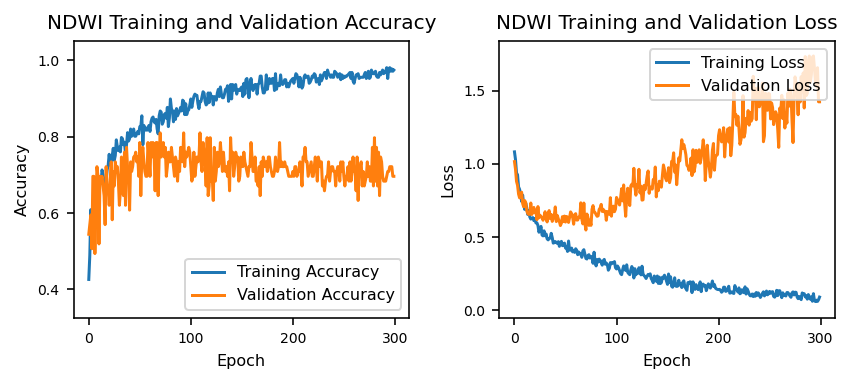
\includegraphics[width=0.5\linewidth]{contents/figures/ME overfitting example.jpg}
    \caption{Overfitting with 300 epoch training}
    \label{fig:ME overfitting}
\end{figure}

\begin{figure}
    \centering
    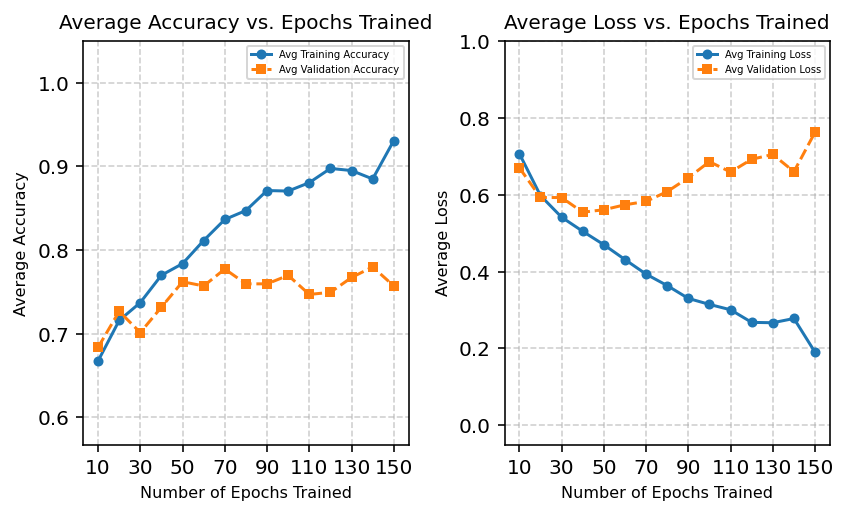
\includegraphics[width=0.5\linewidth]{contents/figures/ME_epoch_pathfinder_better.jpg}
    \caption{10 to 150 epochs 5 times each averaged}
    \label{fig:enter-label}
\end{figure}

\subsubsection{Training Result Visualisation}
Plots the training and validation accuracy and loss curves over epochs using \verb|matplotlib|.
\begin{itemize}
    \item It checks if the \texttt{history} object exists (i.e., if training completed successfully).
    \item Extracts accuracy (\texttt{acc}), validation accuracy (\verb|val_acc|), loss (\texttt{loss}), and validation loss (\verb|val_loss|) from \texttt{history.history}.
    \item Creates a figure with two subplots:
    \begin{itemize}
        \item Left subplot: Plots training vs. validation accuracy against epochs.
        \item Right subplot: Plots training vs. validation loss against epochs.
    \end{itemize}
    \item Adds labels, titles, legends, and adjusts axis limits for clarity.
    \item \verb|plt.tight_layout()| adjusts spacing, and \texttt{plt.show()} displays the plots.
\end{itemize}

\subsubsection{Predicting on New Data}
Uses the trained model to predict the class of a single, predefined test image.
\begin{itemize}
    \item Checks if the \verb|test_image_path| exists.
    \item Loads the test image using \verb|image_to_array| and displays it using \texttt{plt.imshow}.
    \item Loads the same image using \verb|tf.keras.utils.load_img|, resizing it to the model's expected input size (\verb|IMG_HEIGHT|, \verb|IMG_WIDTH|).
    \item Converts the image to a NumPy array (\verb|img_to_array|) and adds a batch dimension (\verb|tf.expand_dims|).
    \item \verb|model.predict()|: Feeds the prepared image array to the trained model to get predictions (\verb|logits|).
    \item \texttt{tf.nn.softmax()}: Converts the output logits into probabilities for each class.
    \item \texttt{np.argmax()}: Finds the index of the class with the highest probability.
    \item Retrieves the corresponding \verb|class_name| using the index.
    \item Calculates the confidence percentage (\texttt{100 * np.max(score)}).
    \item Prints the predicted class name and confidence score. It also includes a simple check to see if the prediction matches the expected class based on the filename (\texttt{"reservoir"}).
\end{itemize}

\subsubsection{Saving and Summary}
Optionally saves the trained model and prints a final summary.
\begin{itemize}
    \item Checks the '\verb|SAVE_MODEL|' flag and if training was successful ('history' exists).
    \item If the target '\verb|model_save_path|' already exists, it creates a new versioned filename by appending a timestamp ('\verb|_YYYYMMDD_HHMMSS|') to avoid overwriting.
    \item '\verb|model.save()|': Saves the entire model (architecture, weights, optimizer state) to the specified path in Keras format ('\verb|.keras|').
    \item Prints the final save path or error messages if saving fails.
    \item Prints the total script execution time.
\end{itemize}

\subsection{KRISP Walk-through}

\subsubsection{Preliminaries}
Imports necessary libraries: time, os, numpy, sys, re (for regex filename parsing), math, matplotlib, tensorflow, keras. Imports custom functions: '\verb|image_to_array|', '\verb|mask_sentinel|', '\verb|save_image_file|', '\verb|split_array|', '\verb|create_9_random_coords|', spinner functions. Sets up the home directory path. Defines '\verb|class_names|'.

\subsubsection{Checking for Pre-Existing Files}
This section manages the generation of small image 'mini-chunks' from the input Sentinel-2 scene, which will be fed into the model for prediction. It includes checks to avoid regenerating data unnecessarily.
\begin{itemize}
    \item Defines the path ('\verb|test_data_path|') where the NDWI mini-chunk images will be saved (e.g., '\verb|test data/ndwi_0.4/|').
    \item Lists existing files in that directory.
    \item Uses \verb|regex| ('\verb|re.compile|') to parse filenames like '\verb|ndwi chunk <i> minichunk <j>.png|' to find the highest chunk index ('\verb|max_chunk_index|') already processed and saved.
    \item Calculates remaining chunks and percentage.
    \item If existing chunks are found, it prompts the user ('input()') whether to continue generating the remaining chunks ('\verb|generate_chunks = True|') or exit ('\verb|sys.exit(0)|'). If no existing files match or the directory doesn't exist, it assumes generation is needed ('\verb|generate_chunks = True|' implicitly or explicitly).
\end{itemize}

\subsubsection{Initial Image Handling (Conditional)}
Note: this step only runs if \verb|generate_chunks| is \verb|True|.

\begin{itemize}
    \item Locates and opens the Green (B03) and NIR (B08) 10m band images from the specified Sentinel-2 folder, similar to NALIRA (steps 3.3.2).
    \item Converts them to NumPy arrays using '\verb|image_to_array|'.
\end{itemize}

\subsubsection{Cloud Masking (Conditional)}
Note: this step only runs if \verb|generate_chunks| is \verb|True|.

\begin{itemize}
    \item Applies cloud masking using the 20m cloud probability file, upscaling the mask to 10m resolution, similar to NALIRA (step 3.3.3). The function '\verb|mask_sentinel|' modifies the '\verb|image_arrays|' (Green, NIR) in place.
\end{itemize}

\subsubsection{Calculating NDWI (Condtional)}
Note: this step only runs if \verb|generate_chunks| is \verb|True|.

Calculates the NDWI array from the masked Green and NIR arrays, similar to NALIRA (step 3.3.4).

\subsubsection{True Colour Image Handling (Optional)}
Note: this step only runs if \verb|generate_chunks| is \verb|True|. 

\subsubsection{Generating Chunks and Saving Images (Conditional)}
Note: this step only runs if \verb|generate_chunks| is \verb|True|.

\begin{figure}
    \centering
    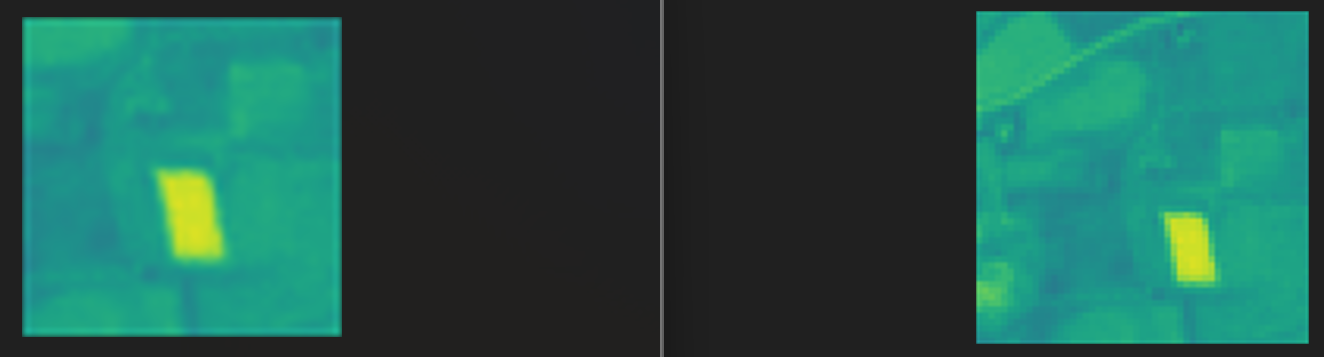
\includegraphics[width=0.5\linewidth]{contents/figures/ME different way of making images.jpg}
    \caption{Different ways of making images (array conversion vs direct image crop) has effects on aliasing}
    \label{fig:ME different image methods}
\end{figure}

\begin{itemize}
    \item Splits the full NDWI array into '\verb|n_chunks|' using '\verb|split_array|'.
    \item Determines the global minimum and maximum NDWI values across all chunks (max is scaled by '\verb|max_multiplier|').
    \item Iterates through the NDWI chunks ('\verb|ndwi_chunks|'). If resuming, it skips chunks with index less than '\verb|start_chunk_index|'.
    \item For each chunk '\verb|i|':
    \begin{itemize}
        \item '\verb|create_9_random_coords|': Generates coordinates for 9 slightly overlapping mini-chunks within the current chunk.
        \item For each mini-chunk coordinate set 'j':
        \begin{itemize}
            \item Defines the output image name (e.g., 'ndwi chunk i minichunk j.png').
            \item '\verb|save_image_file|': Saves the mini-chunk region from the parent NDWI chunk 'i' as a normalised PNG image file in the '\verb|test_data_path|'. Normalization uses the pre-calculated global min/max. '\verb|dupe_check|' is \verb|False| as overwriting might be intended if resuming.
        \end{itemize}
    \end{itemize}
\end{itemize}

\subsubsection{Model Deployment}
Loads the pre-trained model and uses it to classify the generated (or pre-existing) NDWI mini-chunk images.
\begin{itemize}
    \item Load model
    \begin{itemize}
        \item Defines the path to the saved Keras model file ('\verb|model_path|') based on 'HOME', 'IPDMP', '\verb|saved_models|', and the specified '\verb|model_name|'.
        \item '\verb|keras.models.load_model()|': Loads the trained model architecture and weights.
    \end{itemize}
    \item Prediction Loop
    \begin{itemize}
        \item Gets a list of all mini-chunk image filenames from the '\verb|test_data_path|' (limited to the first 20 in the provided code for demonstration).
        \item Iterates through each '\verb|file_name|':
        \begin{itemize}
            \item Constructs the full '\verb|file_path|'.
            \item '\verb|tf.keras.utils.load_img()|': Loads the mini-chunk image, resizing it to the model's expected input dimensions ('height', 'width' - e.g., 157x157).
            \item Displays the loaded mini-chunk image using 'plt.imshow'.
            \item '\verb|tf.keras.utils.img_to_array()|': Converts the image to a NumPy array.
            \item '\verb|tf.expand_dims()|': Adds a batch dimension.
            \item 'model.predict()': Feeds the prepared image array to the loaded model, obtaining prediction logits.
            \item 'tf.nn.softmax()': Converts logits to class probabilities.
            \item 'np.argmax()': Finds the index of the highest probability class.
            \item Retrieves the corresponding '\verb|predicted_class_name|' from '\verb|class_names|'.
            \item Calculates the 'confidence' percentage.
            \item Prints the prediction result (class name and confidence) for the mini-chunk image.
        \end{itemize}
    \end{itemize}
\end{itemize}

\section{NALIRA User Interface}
\begin{figure}
     \centering
     \begin{subfigure}[b]{0.3\textwidth}
         \centering
         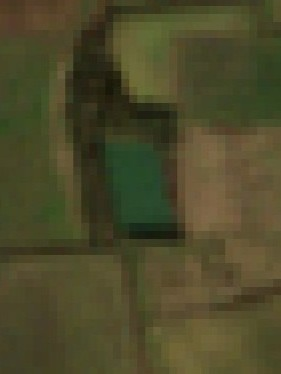
\includegraphics[width=\linewidth]{contents/figures/LR 10m res.jpg}
         \caption{User prompted on number of reservoirs}
         \label{fig:ipdgs ui first prompt}
     \end{subfigure}
     \hfill
     \begin{subfigure}[b]{0.3\textwidth}
         \centering
         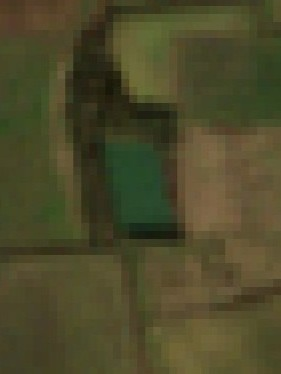
\includegraphics[width=\linewidth]{contents/figures/LR 10m res.jpg}
         \caption{User creating a polygon of the reservoirs' coordinates}
         \label{fig:ipdgs ui polygon}
     \end{subfigure}
     \hfill
     \begin{subfigure}[b]{0.3\textwidth}
         \centering
         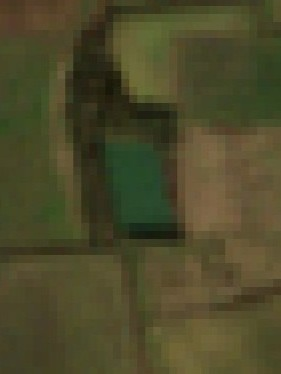
\includegraphics[width=\linewidth]{contents/figures/LR 10m res.jpg}
         \caption{IPDGS automatically generates the next chunk}
         \label{fig:ipdgs ui next chunk}
     \end{subfigure}
        \caption{Example IPDGS User Interface}
        \label{fig:ipdgs ui}
\end{figure}

